\documentclass{article}
\usepackage[margin=1in]{geometry}
\usepackage{enumitem}
\usepackage{setspace}
\usepackage{amsmath}
\usepackage{amssymb}
\usepackage{physics}
\usepackage{relsize}
\usepackage{graphicx}

\title{Math 132 Homework 4}
\date{10/28/2020}
\author{Jiaping Zeng}

\begin{document}
\setstretch{1.35}
\maketitle

\begin{itemize}
    \item [3.2.34] $\abs{\mathlarger{\int_\gamma}e^zdz}\leq\frac{\pi}{4}$, where $\gamma(t)=e^{it},\frac{\pi}{2}\leq t\leq\frac{3\pi}{4}$.\\
          \textbf{Answer}: $L=\ell(\gamma)=r\theta=1\cdot(\frac{3\pi}{4}-\frac{\pi}{2})=\frac{\pi}{4}$; then since $\gamma(t)=e^{it}$, we have $\abs{z}=1$. So $\abs{f(z)}=\abs{e^z}=1=M$. Therefore $\abs{\mathlarger{\int_\gamma}e^zdz}\leq ML=\frac{\pi}{4}$.
    \item [3.2.36] $\abs{\mathlarger{\int_{C_2(0)}}\frac{1}{z-1}dz}\leq 4\pi$.\\
          \textbf{Answer}: $L=\ell(C_2(0))=2\pi r=2\pi\cdot 2=4\pi$; to find $M$, we have $C_2(0)\implies\abs{z}=2$, so $M=2$. Therefore $\abs{\mathlarger{\int_{C_2(0)}}ra\frac{1}{z-1}dz}\leq ML=4\pi$.
    \item [3.2.39] $\abs{\mathlarger{\int_{C_1(0)}}e^{z^2+1}dz}\leq 2\pi e^2$.\\
          \textbf{Answer}: $L=\ell(C_1(0))=2\pi r=2\pi\cdot 1=2\pi$; Then $C_1(0)\implies\abs{z}=1$, so $\abs{f(z)}=\abs{e^{z^2+1}}=e^{\abs{z^2+1}}=e^2=M$. Therefore $\abs{\mathlarger{\int_{C_1(0)}}e^{z^2+1}dz}\leq ML=2\pi e^2$.
    \item [3.3.15] $\mathlarger{\int_{[z_1,z_2,z_3]}}3(z-1)^2dz$, where $z_1=1,z_2=i,z_3=1+i$.\\
          \textbf{Answer}: Let $F(z)=(z-1)^3$, then $F'(z)=3(z-1)^2$. By FTCC, $\mathlarger{\int_{[z_1,z_2,z_3]}}3(z-1)^2dz=F(1+i)-F(1)=i^3-0=-i$.
    \item [3.3.19] $\mathlarger{\int_{[z_1,z_2,z_3]}}ze^zdz$, where $z_1=\pi,z_2=-1,z_3=-1-i\pi$.\\
    \textbf{Answer}: Let $F(z)=ze^z-e^z$, then $F'(z)=ze^z$. By FTCC, $\mathlarger{\int_{[z_1,z_2,z_3]}}ze^zdz=F(-1-i\pi)-F(\pi)=2e^{-1}+i\pi e^{-1}-\pi e^\pi+e^\pi$.
    \item [P1] Find the value of $\mathlarger{\int_{C_1(0)}}z^mdz$ in terms of $m$, where $m\in\mathbb{Z}=\{\ldots,-2,-1,0,1,2,\ldots\}$.\\
          \textbf{Answer}: $C_1(0)\implies\gamma(t)=e^{it},t\in[0,2\pi]$ and $\gamma'(t)=ie^{it}$. Then $\mathlarger{\int_{C_1(0)}}z^mdz=\mathlarger{\int_0^{2\pi}}[\gamma(t)]^m\gamma'(t)dt=\mathlarger{\int_0^{2\pi}}(e^{it})^m\cdot ie^{it}dt=i\mathlarger{\int_0^{2\pi}}e^{it(m+1)}dt=\frac{i}{i(m+1)}[e^{it(m+1)}]_0^{2\pi}=\frac{e^{2i\pi(m+1)}-1}{m+1}$.
    \item [P2] Let $\gamma$ be the clockwise boundary of the wedge \[U=\left\{z\in\mathbb{C}\mid-\frac{3\pi}{4}<\text{Arg }(z)<-\frac{\pi}{2},\text{and }\abs{z}<2\right\}\] Plot $\gamma$ and calculate $\mathlarger{\int_\gamma}\bar{z}dz$.\\
          \textbf{Answer}: We can break $\gamma$ into three parts as follows. Let $\gamma_1=-\frac{\sqrt{2}}{2}t-i\frac{\sqrt{2}}{2}t$ for $t\in[0,1]$, $\gamma_2=2e^{it}$ for $t\in(-\frac{3\pi}{4},-\frac{\pi}{2})$ and $\gamma_3=-2i+2it$ for $t\in[0,1]$. We also have $\gamma_1'(t)=-\frac{\sqrt{2}}{2}-i\frac{\sqrt{2}}{2}$, $\gamma_2'(t)=2ie^{it}$ and $\gamma_3'(t)=2i$. Then,\\
          $\mathlarger{\int_\gamma}\bar{z}dz=\mathlarger{\int_{\gamma_1}}\bar{z}dz+\mathlarger{\int_{\gamma_2}}\bar{z}dz+\mathlarger{\int_{\gamma_3}}\bar{z}dz$\\$=\mathlarger{\int_0^1}\overline{\gamma_1(t)}\gamma_1'(t)dt+\mathlarger{\int_{-\frac{3\pi}{4}}^{-\frac{\pi}{2}}}\overline{\gamma_2(t)}\gamma_2'(t)dt+\mathlarger{\int_0^1}\overline{\gamma_3(t)}\gamma_3'(t)dt$\\$=\mathlarger{\int_0^1}(-\frac{\sqrt{2}}{2}t+i\frac{\sqrt{2}}{2}t)(-\frac{\sqrt{2}}{2}-i\frac{\sqrt{2}}{2})dt+\mathlarger{\int_{-\frac{3\pi}{4}}^{-\frac{\pi}{2}}}2e^{-it}\cdot 2ie^{it}dt+\mathlarger{\int_0^1}2i(2i-2it)dt$\\$=\mathlarger{\int_0^1}tdt+4i\mathlarger{\int_{-\frac{3\pi}{4}}^{-\frac{\pi}{2}}}dt+4\mathlarger{\int_0^1}t-1dt$\\$=\frac{1}{2}+i\pi-2$\\$=-\frac{3}{2}+i\pi$.
          \begin{center}
              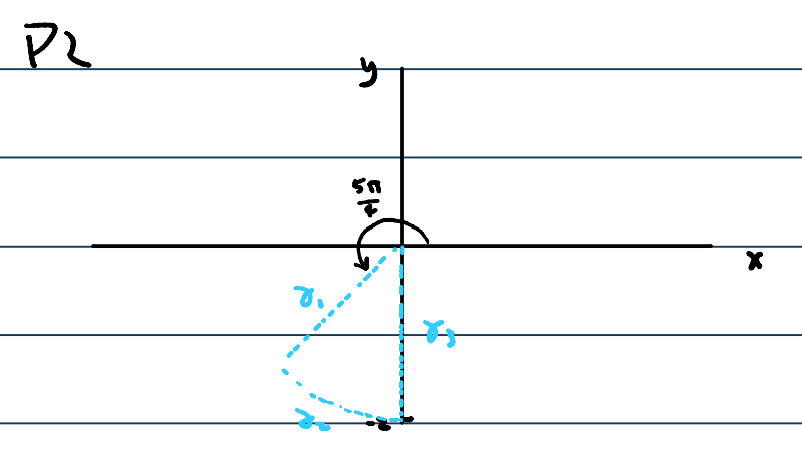
\includegraphics[width=3in]{p2.png}
          \end{center}
    \item [P3] Evaluate $\mathlarger{\int_\gamma}(\sin z+e^z)dz$, where $\gamma$ is the path $[1+i,5-i,2i,-4,\pi+i\sqrt{2},41-41i,10^{10}+i,\pi]$.\\
          \textbf{Answer}: Let $F=e^z-\cos z$, then $F'(z)=e^z+\sin z$. By FTCC, $\mathlarger{\int_\gamma}(\sin z+e^z)dz=F(\pi)-F(1+i)=\sin\pi+e^\pi-\sin(1+i)-e^{1-i}=e^\pi-e^{1-i}-\sin(1+i)$.
\end{itemize}
\end{document}